We evaluate the proposed approach with four experiments.
A toy problem is first used to study the transfer of learning between two related processes via the shared inducing points.
We then compare the model with existing multioutput models on the tasks of predicting foreign exchange rate and air temperature.
In the final experiment, we show that joint learning under sparsity can lead to significant performance gain on a large scale dataset of inverse dynamics of a robot arm. 

Since we are using stochastic optimization, the learn rates need to be chosen carefully.
We found that the rates used in \citep{hensmangaussian} also work well for our model.
Specifically, we used the learn rates of $0.01$ for the variational parameters, $1 \times 10^{-5}$ for the  covariance hyperparameters, and $1 \times 10^{-4}$ for the weights, noise hyperparameter, and inducing inputs.
We also included a momentum term of $0.9$ for all of the parameters except the variational parameters and the inducing inputs.
All of the experiments are executed on an Intel(R) Core(TM) i7-2600 3.40GHz CPU with 8GB of RAM using Matlab R2012a.

\subsection{TOY PROBLEM}
In this toy problem, two related outputs are simulated from the same latent function $sin(x)$ and corrupted by independent noises: $y_1(x) = sin(x) + \epsilon$ and $y_2(x) = -sin(x) + \epsilon$, $\epsilon \sim \Normal(0,0.01)$.
Each output is given 200 observations with missing values in the $(-7,-3)$ interval for the first output and the $(4,8)$ interval for the second output.
We used $Q = 1$ latent sparse process, $h_1(x) = h_2(x) = 0$, $M = 15$ inducing inputs for our model.

Figure \ref{fig:toy} shows the predictive distributions by COGP and independent GPs with stochastic variational inference (SVIGP, one for each output).
The locations of the inducing inputs are fixed and identical for both methods.
It is apparent from the figure that the independent GPs fail to predict the functions in the unobserved regions, especially for output 1.
In contrast, prediction by COGP is perfect in these regions by using information from the observed intervals of one output to interpolate the missing signal of the other.
Thus, this confirms the effectiveness of collaborative learning of sparse processes via the shared inducing variables. 
Also note that the inference procedure learned that the weights are $w_{11} = 1.07$ and $w_{21} = -1.06$ which accurately reflects the correlation between the two outputs.

\begin{figure*}
\centering
\begin{tabular}{cccc}
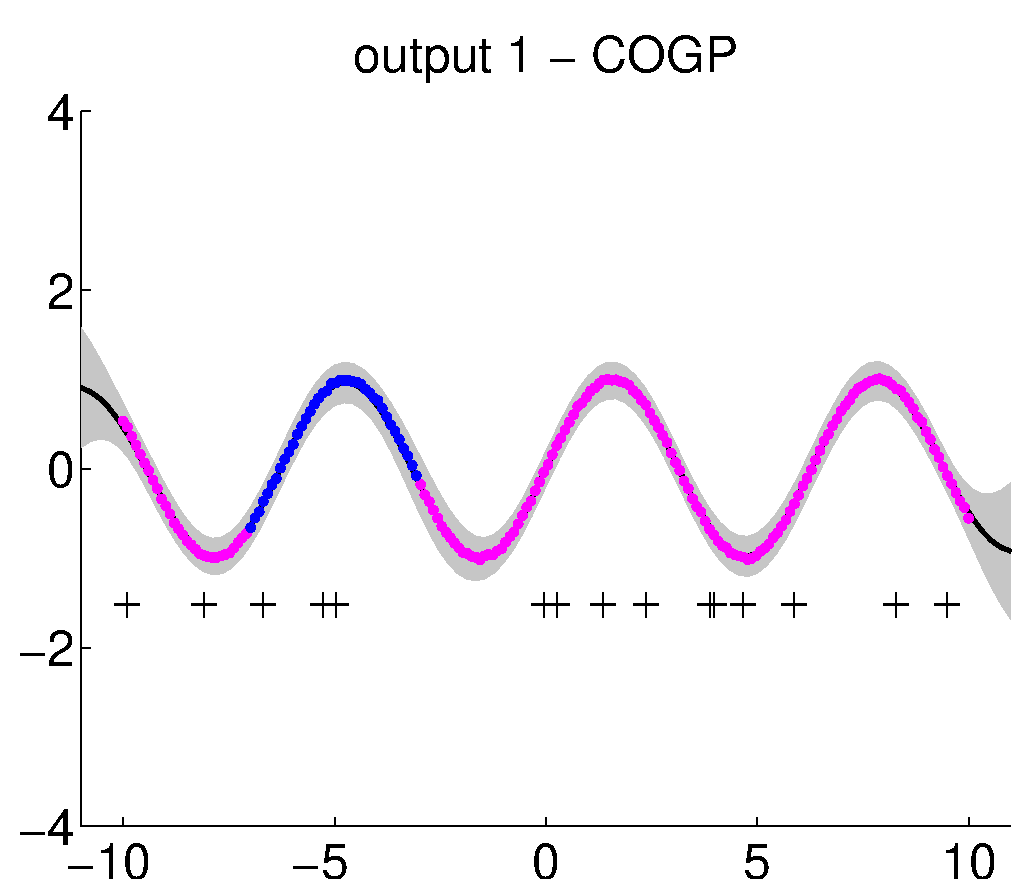
\includegraphics[scale=0.2]{figures/toy-slfm-y1.eps} &
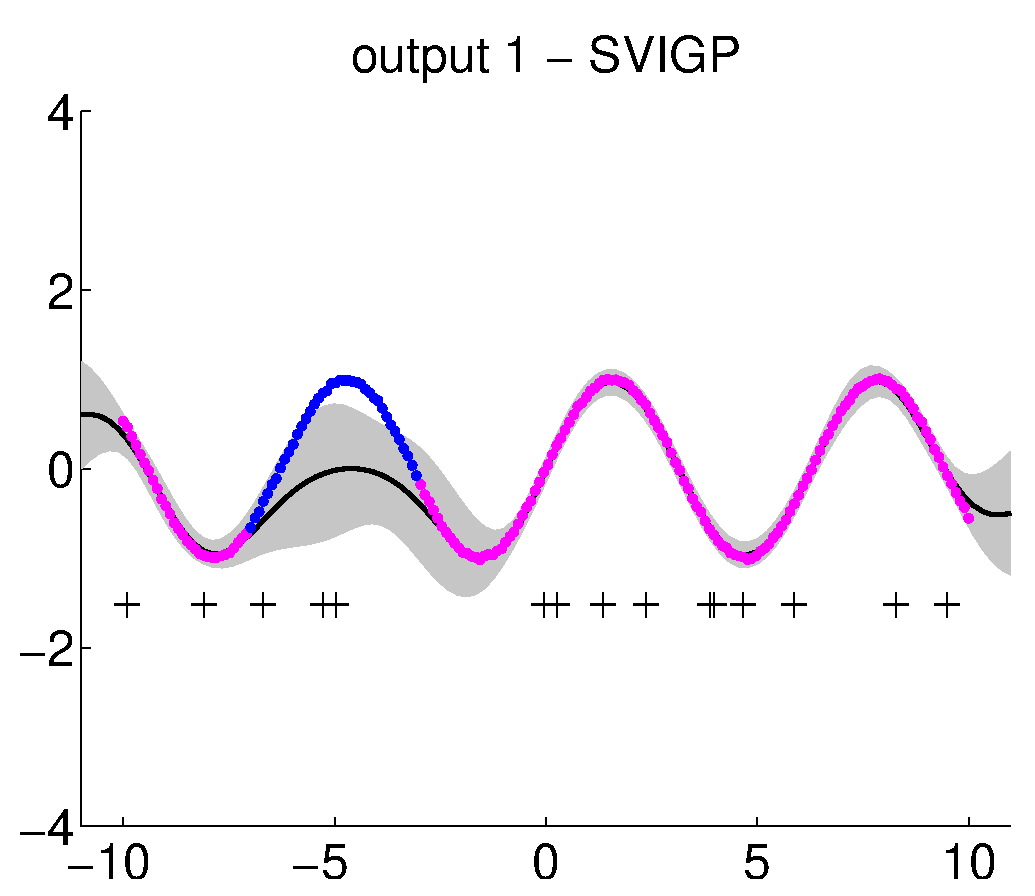
\includegraphics[scale=0.2]{figures/toy-svigp-y1.eps} &
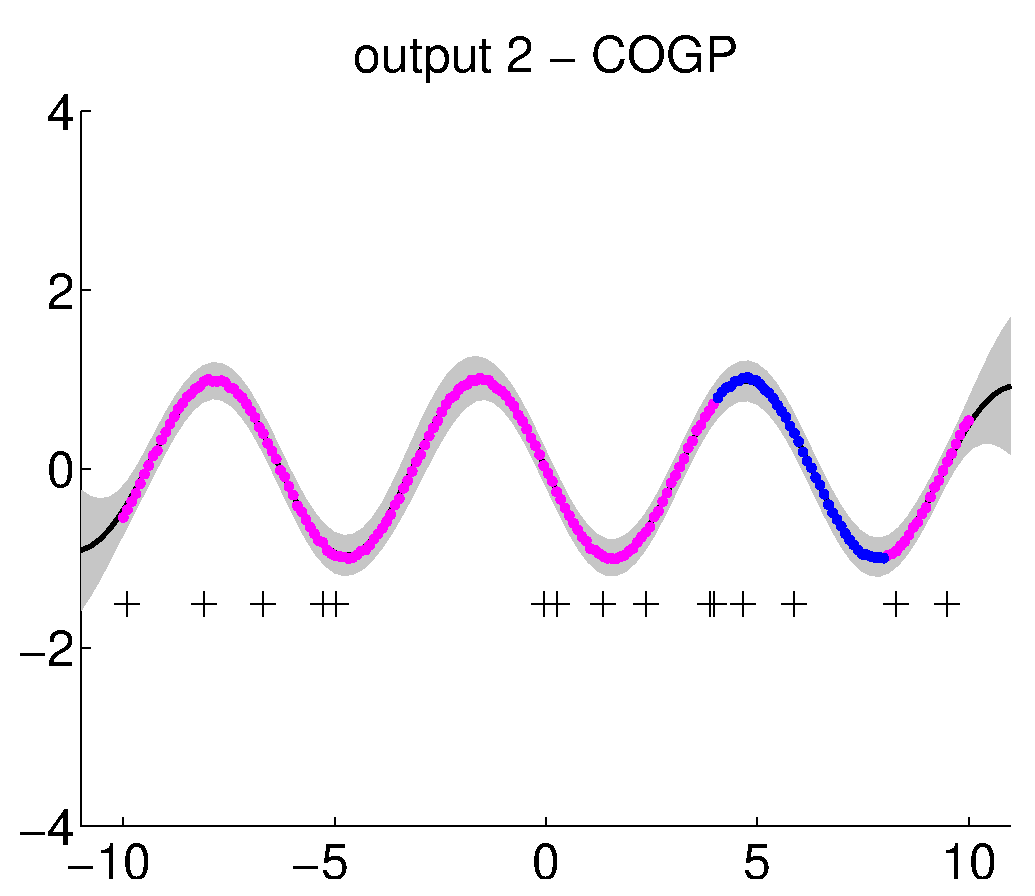
\includegraphics[scale=0.2]{figures/toy-slfm-y2.eps} &
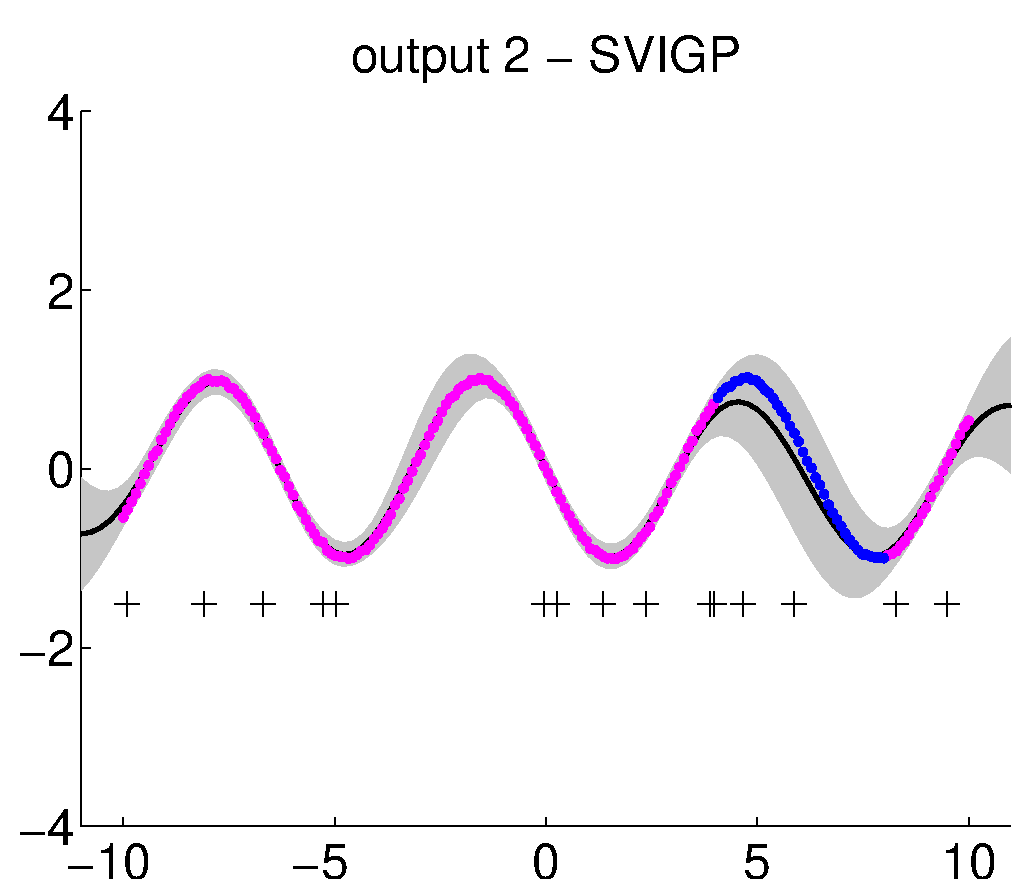
\includegraphics[scale=0.2]{figures/toy-svigp-y2.eps}
\end{tabular}
\caption{Real data and predictive distributions of by COGP (first and third figure) and independent GPs using stochastic variational inference (second and last figure) for the toy problem. Solid black line: predictive mean; grey bar: two standard deviations; magenta dots: real observations; blue dots: missing data. The black crosses show the locations of the inducing inputs. By sharing inducing points across the outputs, COGP accurately interpolates the missing function values.}
\label{fig:toy}
\end{figure*}

\subsection{FOREIGN EXCHANGE RATE PREDICTION}
The first real world application we consider is to predict the foreign exchange rate w.r.t the US dollar of the top 10 international currencies (CAD, EUR, JPY, GBP, CHF, AUD, HKD, NZD, KRW, and MXN) and 3 precious metals (gold, silver, and platinum)\footnote{Data is available at http://fx.sauder.ubc.ca}. 
The setting of our experiment described here is identical to that in \citep{alvarez2010efficient}.
The dataset consists of all the data available for the 251 working days in the year of 2007.
There are 9, 8, and 42 days of missing values  for gold, silver, and platinum, respectively.
We remove from the data the exchange rate of CAD on days 50-100, JPY on day 100-150, and AUD on day 150-200.
Note that these 3 currencies are from very different geographical locations, making the problem more interesting. 
The 153 points are used for testing, and the remaining 3051 data points are used for training.
Since the missing data corresponds to long contiguous sections, the objective here is to evaluate the capacity of the model to impute the missing currency values based on other currencies.
%todo: batch size, learn rate (maybe at the beginning of experiments)

For preprocessing we normalized the outputs to have zero mean and unit variance.
Since the exchange rates are driven by a small number of latent market forces \citep{alvarez2010efficient}, we tried different values of $Q = {1,2,3}$ and selected $Q = 2$ which gave the best model evidence (ELBO).
We used the squared-exponential covariance function for the shared processes and the noise covariance function for the independent process of each output.
The inducing inputs $(M = 100, \text{per sparse process})$  are randomly selected from the training data and fixed throughout training.

The real data and predictive distributions by our model are shown in Figure \ref{fig:fx}.
They exhibit similar behaviors to those by the convolved model with inducing kernels in \citep{alvarez2010efficient}.
In particular, both models perform better at capturing the strong depreciation of the AUD than the fluctuations of the CAD and JPY currency.
Our investigation of the dataset found that 4 other currencies (GBP, NZD, KRW, and MXN) also experienced the same trend during the days 150 - 200.
This was effectively used by the model to extrapolate the values of the AUD.

%todo: result for independent gps
We also report in Table \ref{tab:fx} the predictive accuracy of our model compared to the convolved GPs model with exact inference \citep{alvarez-lawrence-nips-08} (CGP) and with approximation via the variational inducing kernels \citep{alvarez2010efficient}) (CGPVAR) in addition to using independent GPs (IGP, one for each output).
Our model outperforms both of the CGP variants in terms of standardized mean squared error (SMSE).
It has lower test likelihood, as measured by the negative log predictive density (NLPD), which is mainly due to the less conservative predictive variance of the exact CGP for the CAD currency.
%The results are averaged across the 3 outputs over 5 repetitions.
% no std because there are 3 outputs but variance is small
Note that the SMSE of CGPVAR is taken from \citep{alvarez2010efficient} while the NLPD was not provided.
Training took only 10 minutes for our model compared to 1.4 hours for the full CGP model.

\setlength{\tabcolsep}{4pt}
\begin{table}[t]
\caption{Performance comparison on the foreign exchange rate dataset. Results are averaged of the 3 outputs over 5 repetitions.}
\label{tab:fx}
\begin{center}
\begin{tabular}{ccc}
\toprule
\textbf{METHOD} & \textbf{SMSE} & \textbf{NLPD} \\ \hline
COGP  & \textbf{0.2125} & -0.8394 \\
CGP & 0.2427 & \textbf{-2.9474} \\
IGP & 0.5996 & 0.4082 \\
CGPVAR & 0.2795 & NA \\
%ICM & 0.3927 &
\bottomrule
\end{tabular}
\end{center}
\end{table}

\begin{figure*}
\centering
\begin{tabular}{ccc}
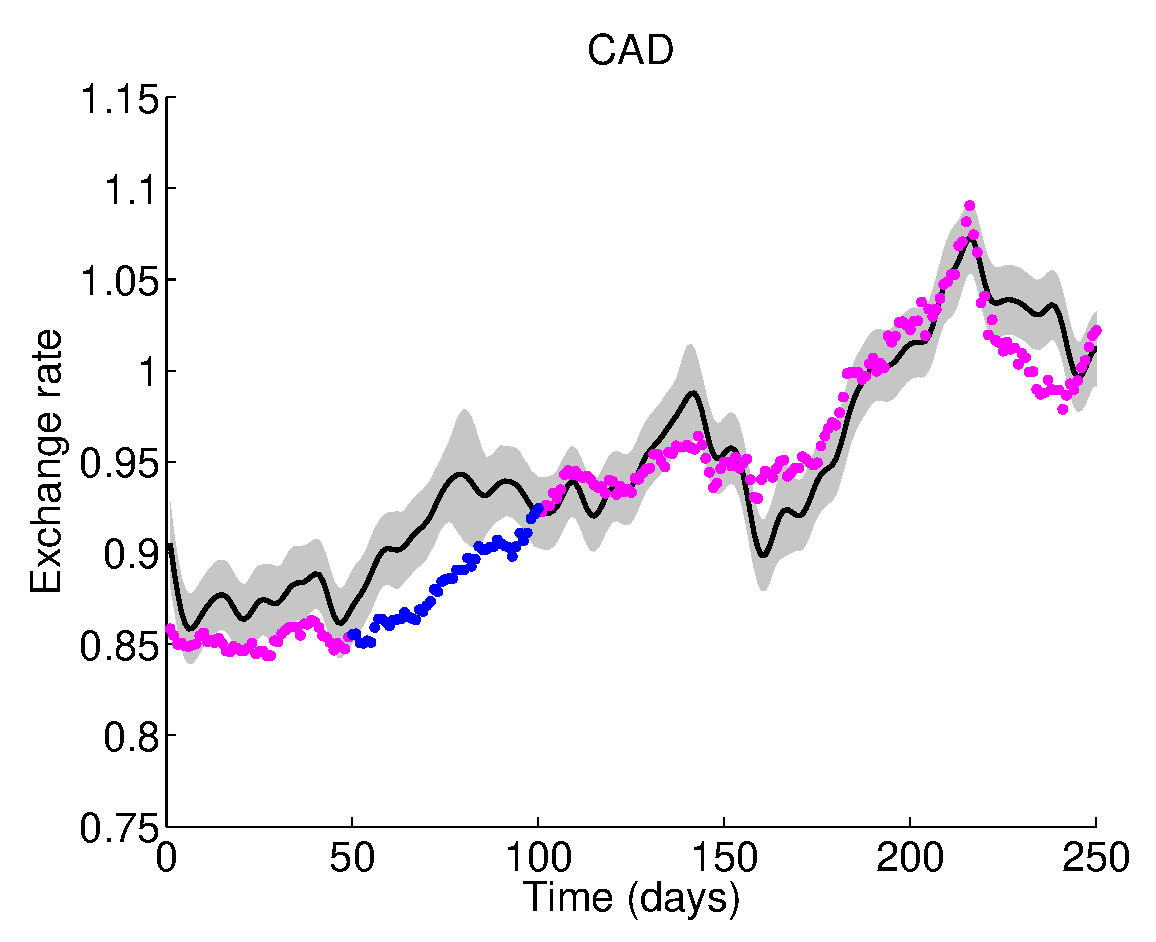
\includegraphics[scale=0.3]{figures/fxCAD.eps} &
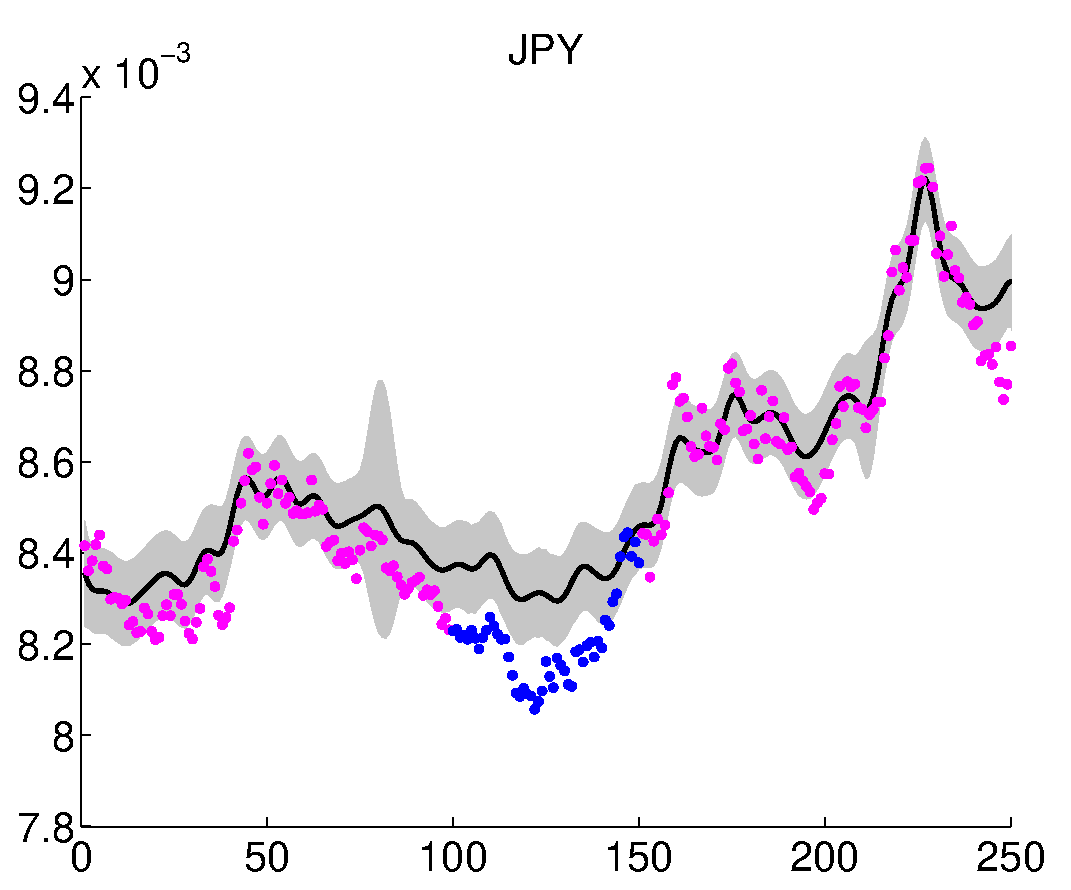
\includegraphics[scale=0.3]{figures/fxJPY.eps} &
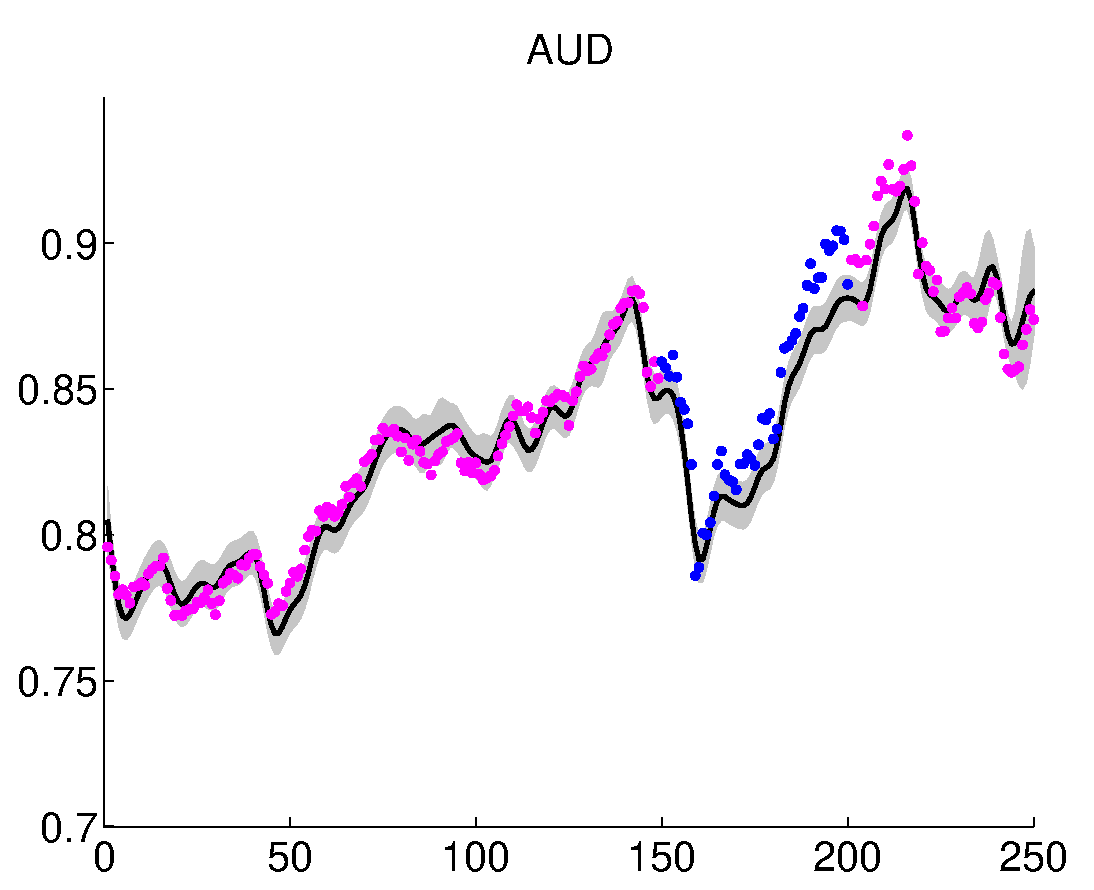
\includegraphics[scale=0.3]{figures/fxAUD.eps}
\end{tabular}
\caption{Real observations and predictive distributions for CAD (left), JPY (middle), and AUD (right). The color coding scheme is the same as in Figure \ref{fig:toy}.}
\label{fig:fx}
\end{figure*}

\subsection{AIR TEMPERATURE PREDICTION}
Next, we consider the task of predicting air temperature at 4 different locations in the south coast of England. 
The data is gathered from a network of weather sensors (named Bramblemet, Sotonmet, Cambermet, and Chimet), each of which measures several environmental variables \citep{osborne2008towards}\footnote{Data is available at seperate web pages, see e.g. http://www.bramblemet.co.uk}.
%The sensors are close geographically so we can expect correlation in air temperature.
We selected the sensor signal for air temperature during the period from July 10 to July 15, 2013.
The sensors record measurements every 5 minutes, resulting in a maximum of 4320 observations.
There are missing data for Bramblemet (100 points), Chimet (15 points), and Sotonmet (1002 points), possibly due to network outages or hardware failures.
We further simulated failure of the sensors by removing the observations from the time periods [10.2 - 10.8] for Cambermet and [13.5 - 14.2] for Chimet.
The removed data comprises 375 data points, which is used for testing, and the remaining data consisting of 15,788 points is used for training.
Similar to the previous experiment, the objective is to evaluate the ability of the model to use the signals from the functioning sensors to extrapolate the missing signals.

For pre-processing we normalized the outputs to have zero mean and unit variance.
The inducing inputs $(M = 200)$ are randomly selected from the training set and fixed throughout training.
The number of latent processes is $Q = 2$ for both our model and the CGP model.

The real data and the predictive distributions by 3 models (COGP, CGP with exact inference \citep{alvarez-lawrence-nips-08}, and independent GPs) are shown in Figure \ref{fig:weather}.
It is clear that the independent GPs model is clueless in the test regions and thus simply uses the average temperature as its prediction.
For Cambermet, both COGP and CGP can capture the rising in temperature from the morning till the afternoon and the fall afterward.
For Chimet, both models perform poorly but CGP more so as it falsely predicts  wild fluctuations that are non-existent in the data. 
Note that the two latent processes learned by our model indeed correspond to different patterns in the data: one process has the inverse lengthscale of 136 which captures the global increase in temperature during the training period while the other has the inverse lengthscale of 0.5 to model the local variations within a single day.
The comparative performance of the models are summarized in Table \ref{tab:air}, from which it can be seen that our model outperforms CGP in terms of both test accuracy and confidence.
%All results are averaged of the 2 outputs over 5 repetitions.
It took 5 minutes on average to train our model compared to 3 hours of CGP with exact inference.

\setlength{\tabcolsep}{4pt}
\begin{table}[t]
\caption{Performance comparison on the air temperature dataset. Results are averaged of 2 outputs over 5 repetitions. }
\label{tab:air}
\begin{center}
\begin{tabular}{ccc}
\toprule
\textbf{METHOD} & \textbf{SMSE} & \textbf{NLPD} \\
\hline
COGP & \textbf{0.1077} & \textbf{2.1712} \\
CGP & 0.1125 & 2.2219 \\
IGP & 0.8944 & 12.5319 \\
\bottomrule
\end{tabular}
\end{center}
\end{table}

\begin{figure*}
\centering
\begin{tabular}{ccc}
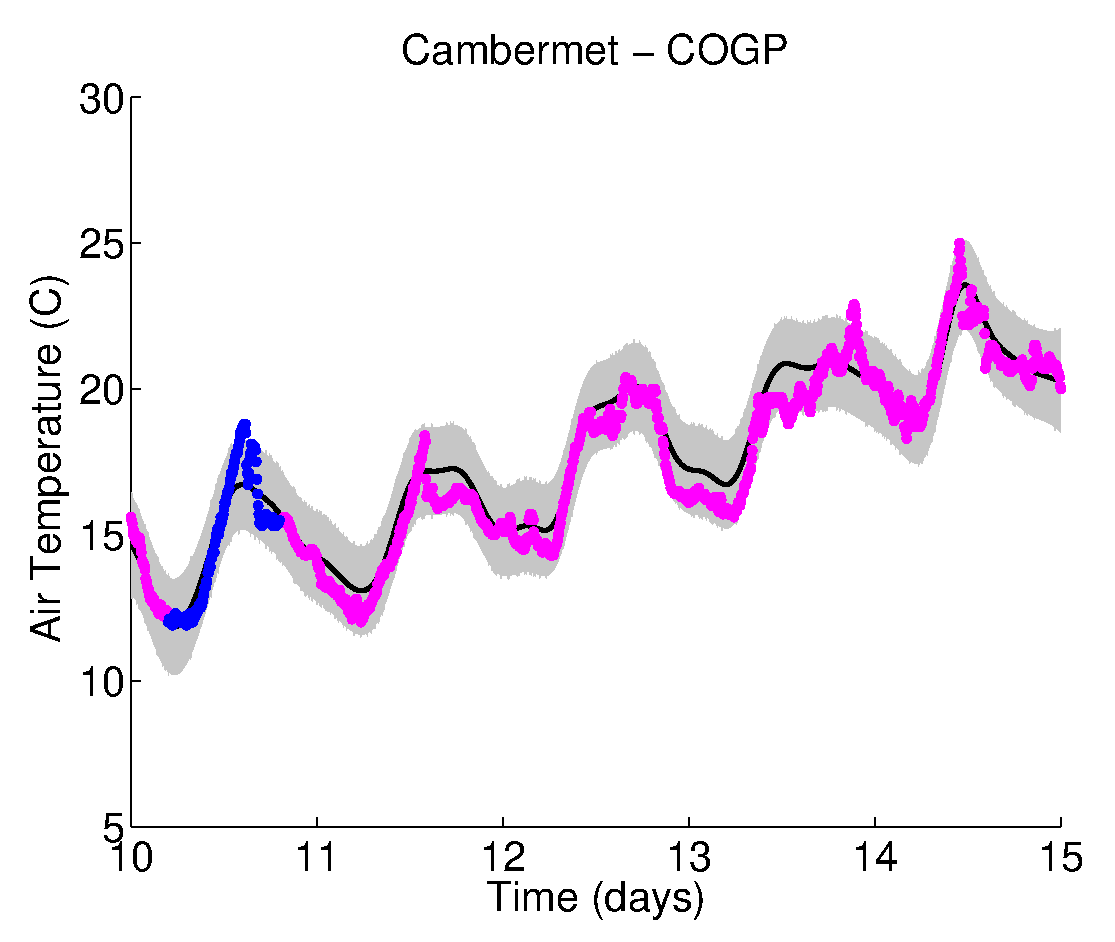
\includegraphics[scale=0.3]{figures/cogp-weatherCambermet.eps} &
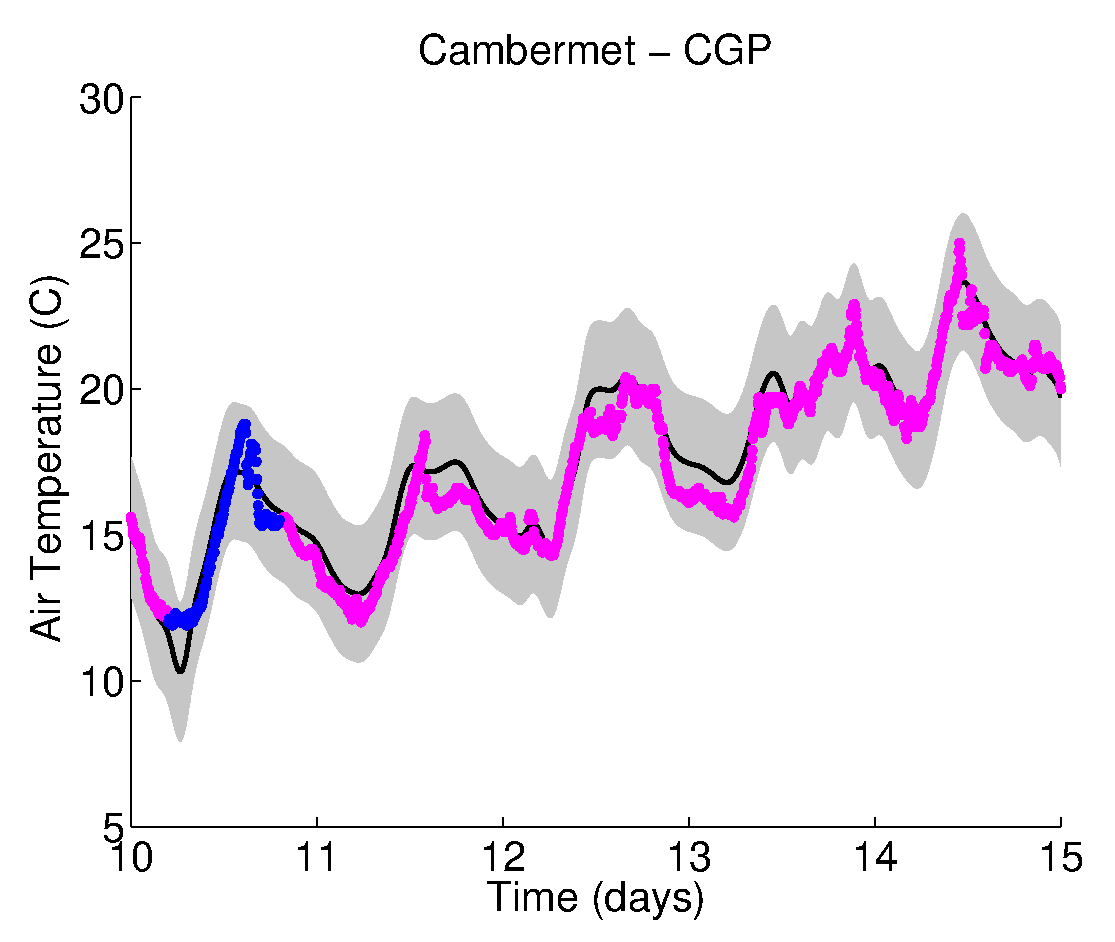
\includegraphics[scale=0.3]{figures/cgp-weatherCambermet.eps} &
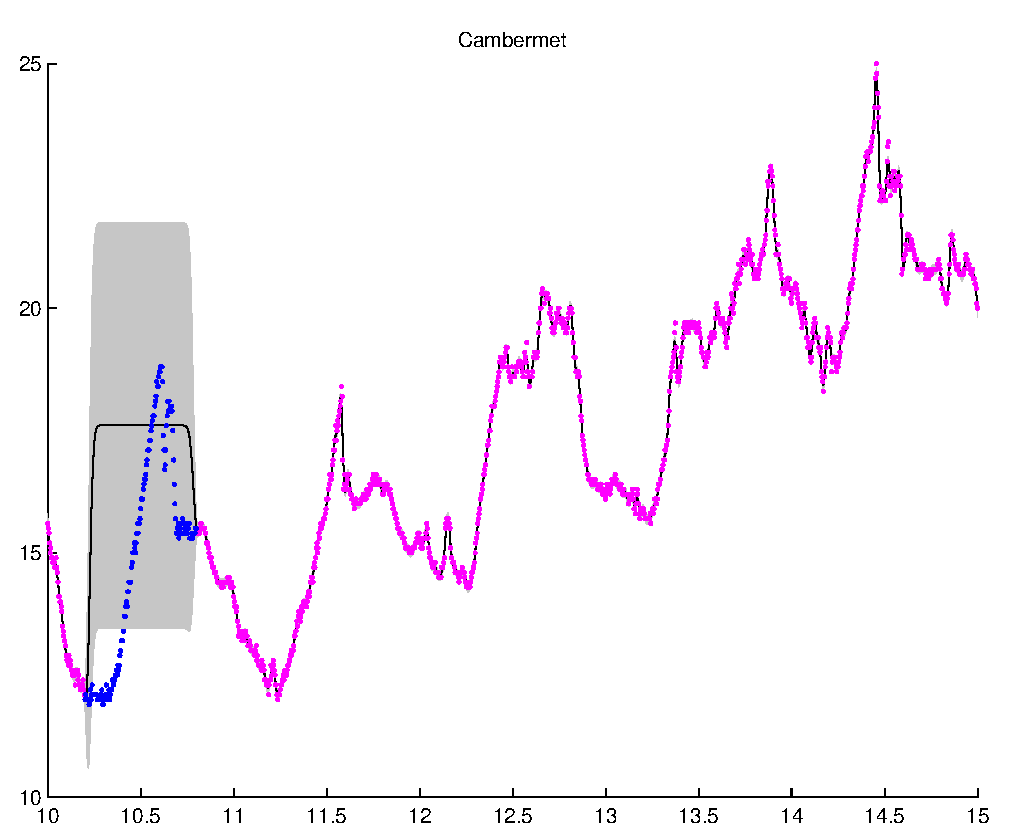
\includegraphics[scale=0.3]{figures/weatherCambermet.eps}
\\
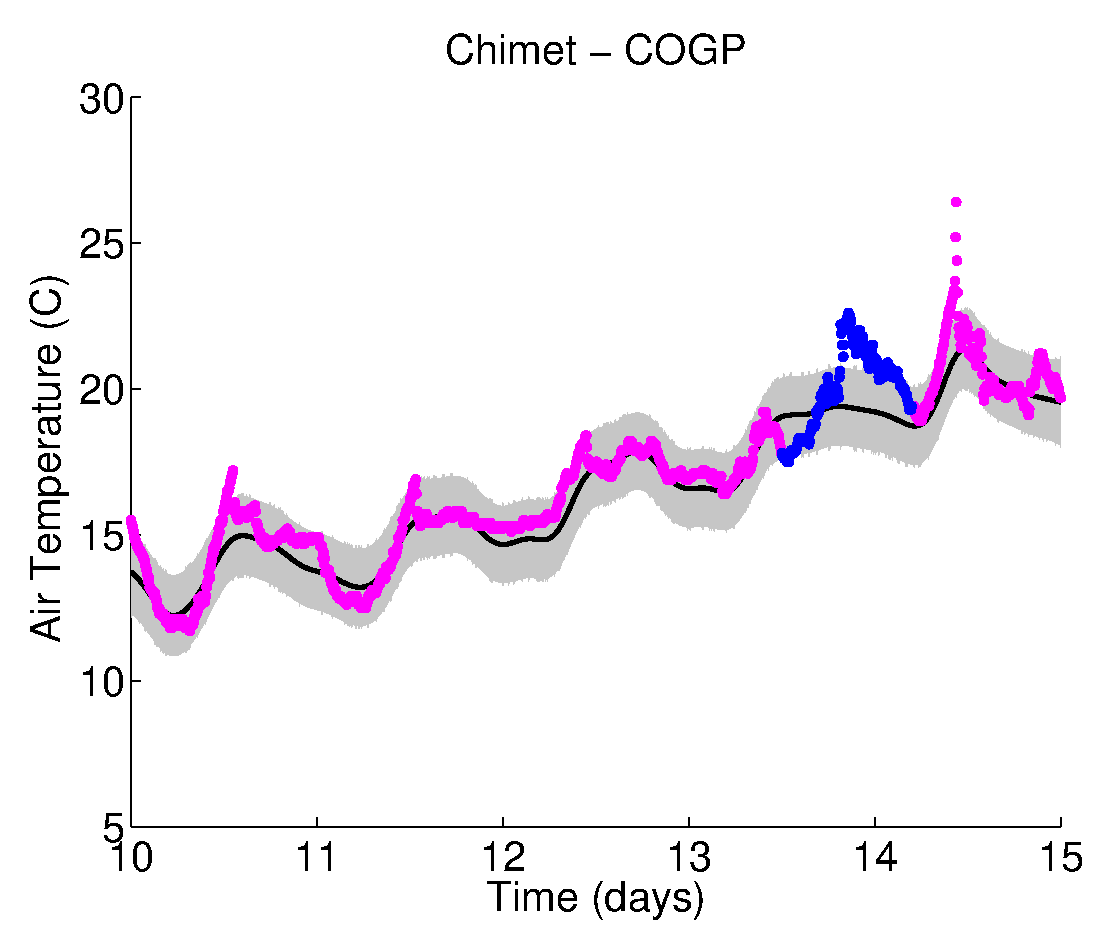
\includegraphics[scale=0.3]{figures/cogp-weatherChimet.eps} &
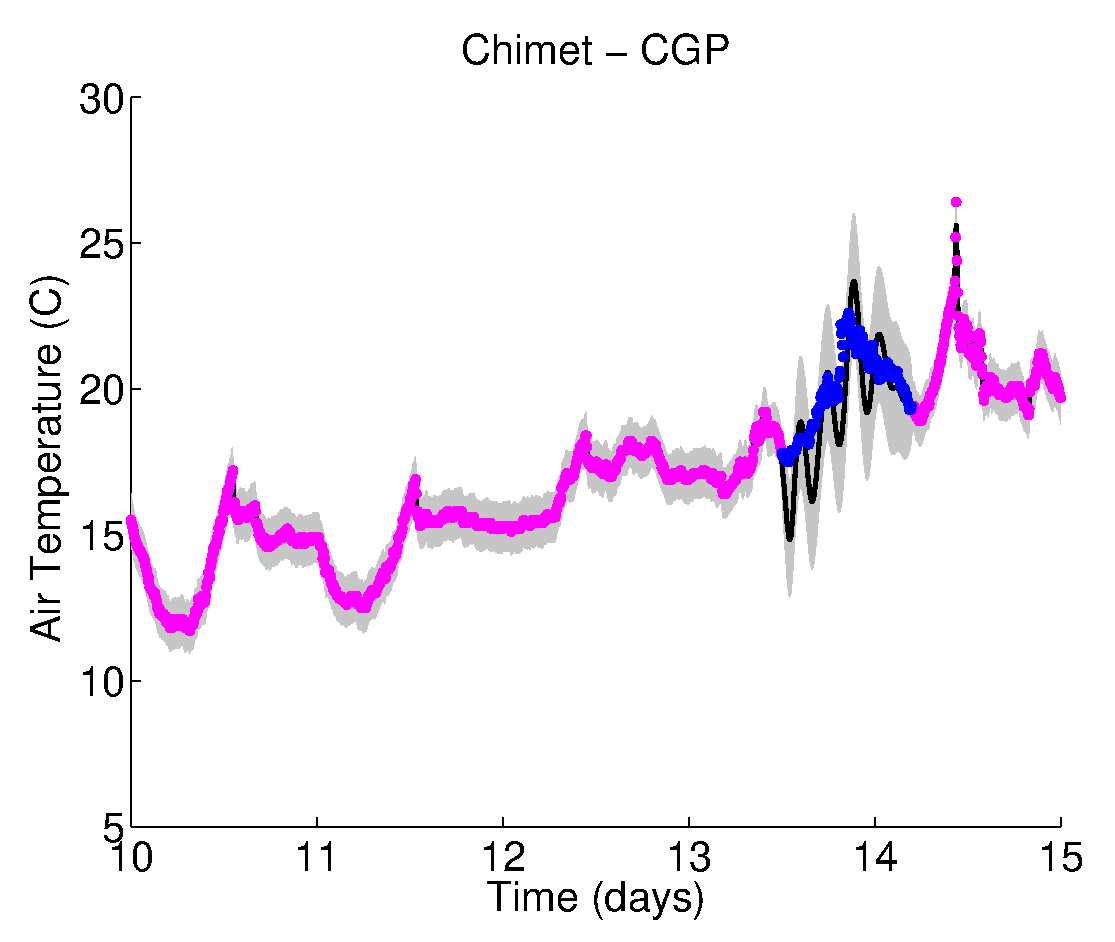
\includegraphics[scale=0.3]{figures/cgp-weatherChimet.eps} &
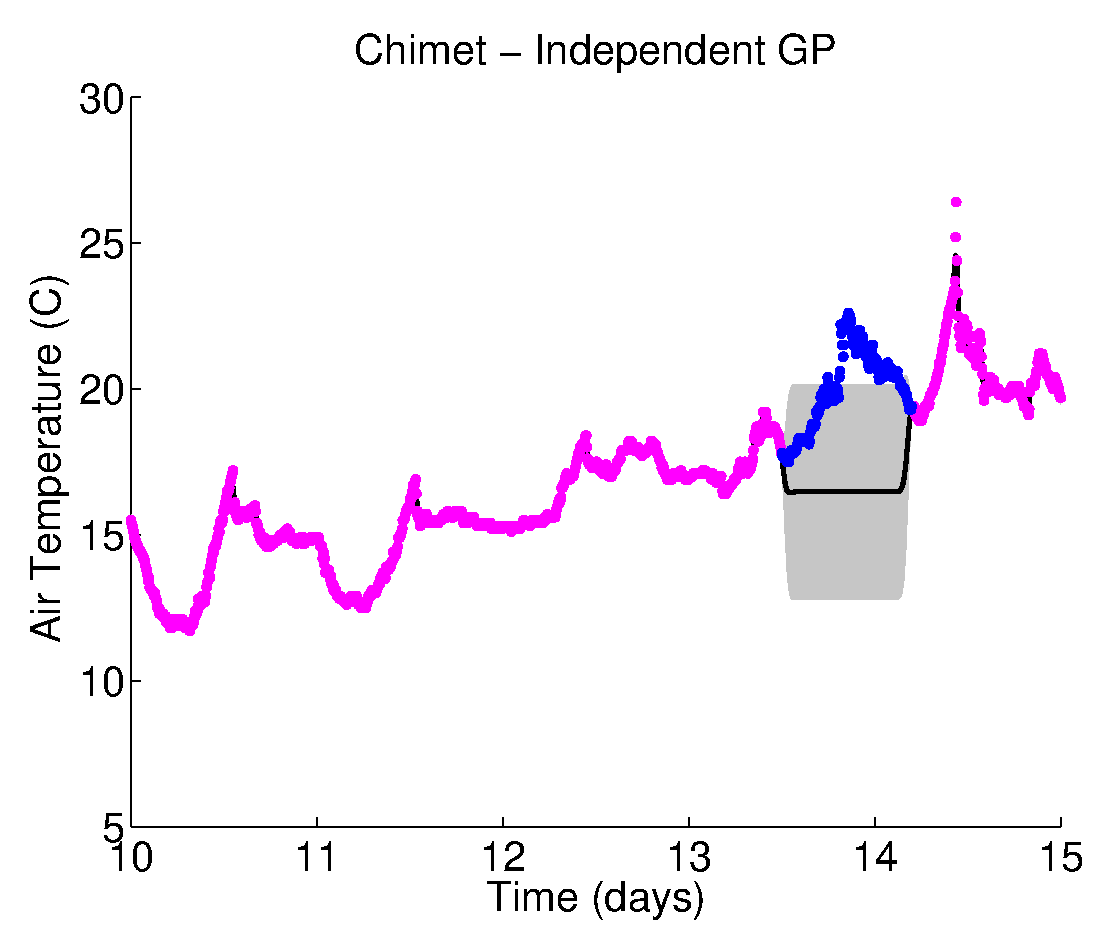
\includegraphics[scale=0.3]{figures/weatherChimet.eps}
\end{tabular}
\caption{Real data and predictive distributions by our method (COGP, left figures), the convolved GP method with exact inference (CGP, middle figures), and full independent GPs (right figures) for the air temperature problem. The color coding is the same as in Figure \ref{fig:toy}}
\label{fig:weather}
\end{figure*}

\subsection{INVERSE DYNAMICS OF ROBOT ARM}
Our last experiment is with a dataset relating to an inverse dynamics model of a 7-degree-of-freedom anthropomorphic robot arm\footnote{Data is available at http://www.gaussianprocess.org/gpml/data/}.
The data consists of 48,933 mapping from a 21-dimensional input space (7 joints positions, 7 joint velocities, 7 joint accelerations) to the corresponding 7 joint torques.
%The problem is strongly nonlinear due to complex superpositions of sine and cosine functions in robot dynamics \citep{vijayakumar2000locally}.
%Furthermore, exploratory analysis using standard GP with automatic relevance determination suggests that all of the 21 dimensions are relevant.
It has been used in previous work (see e.g. \citep{rasmussen-williams-book},  \citep{vijayakumar2000locally}) but only for single task learning.
Here we consider joint learning for the 4th and 7th torques where the first has only 2,000 points  while the second has the full data of 44,484 points for training.
The test set consists of 8,898 observations equally divided between the two outputs.
Note that the data was collected at 100Hz for 7.5 minutes in total, hence ideal for this experiment which evaluates the effectiveness of collaborative learning under the assumption of sparsity in the output spaces.

Since none of the existing multioutput models are applicable to problems of this scale, we compare with independent models that learn each output separately.
Standard GP is applied to the first output as it has only 2,000 observations for training.
For the second output, we used two baselines.
The first is the subset of data (SOD) approach where 2,000 data points are randomly selected for training with a standard GP model.
The second is the sparse GP with stochastic variational inference (SVIGP) using 500 inducing inputs and a batch size of 1,000.
In case of COGP, we also used a batch size of 1,000 and 500 inducing points for the shared process ($Q = 1$) and each of the independent processes.
The squared exponential with automatic relevance determination (SEard) covariance function is used for all processes of all methods.
Finally, the outputs are normalized to have zero mean and unit variance. 

The performance of all methods, in terms of SMSE and NLPD averaged over 5 repetitions, is given in Table \ref{tab:robotarm}.
The benefits of learning the two outputs jointly are evident, as can be seen by the significantly higher test accuracy and confidence of COGP compared to the full GP for the first output (4th torque).
While the SMSE of the second output is essentially the same by all methods, the predictive likelihood of our multioutput model is better than that of the independent SVIGP model which has the same amount of training data for this torque.
The results thus confirm the impact of collaborative learning even when sparsity assumption is made in the model.

\begin{table}[t]
\caption{Performance comparison on the robot arm dataset. In the two bottom lines, standard GP is applied to output 1 and the remaining method is applied to output 2. Results are averaged over 5 repetitions.}
\label{tab:robotarm}
\begin{center}
\begin{tabular}{lcccc}
\toprule
& \multicolumn{2}{c}{\textbf{OUTPUT 1}} & \multicolumn{2}{c}{\textbf{OUTPUT 2}} \\ \cmidrule(r){2-5}
\textbf{METHOD} & \textbf{SMSE} & \textbf{NLPD} & \textbf{SMSE} & \textbf{NLPD}\\ 
 \midrule
COGP, learn z & \textbf{0.2631} & \textbf{3.0600} & 0.0127 & \textbf{0.8302} \\
COGP, fix z & 0.2821& 3.2281 & 0.0131 & 0.8685 \\
GP, SVIGP & 0.3119 & 3.2198 & \textbf{0.0101} & 1.1914 \\
GP, SOD & 0.3119 & 3.2198 & 0.0104 & 1.9407 \\
\bottomrule
\end{tabular}
\end{center}
\end{table}

Also from Table \ref{tab:robotarm}, it seems that optimizing the inducing inputs can lead to better performance than fixing them.
More importantly, this comes with slight overhead in computation, as demonstrated by the training time for the two options in Figure \ref{fig:time}.
For instance, the total training time with 500 inducing inputs is 1.9 hours for learning versus 1.6 hours for keeping them fixed.
Recall that this dataset is 21-dimensional so this confirms our analysis in the inference section that the cost of optimization of the inducing inputs does not scale linearly with the dimensionality of the problem.
Thus, for datasets of high dimension like this one, learning of the inducing inputs is a practical option.

% table for smses, nlpds, training tiem
\begin{figure}
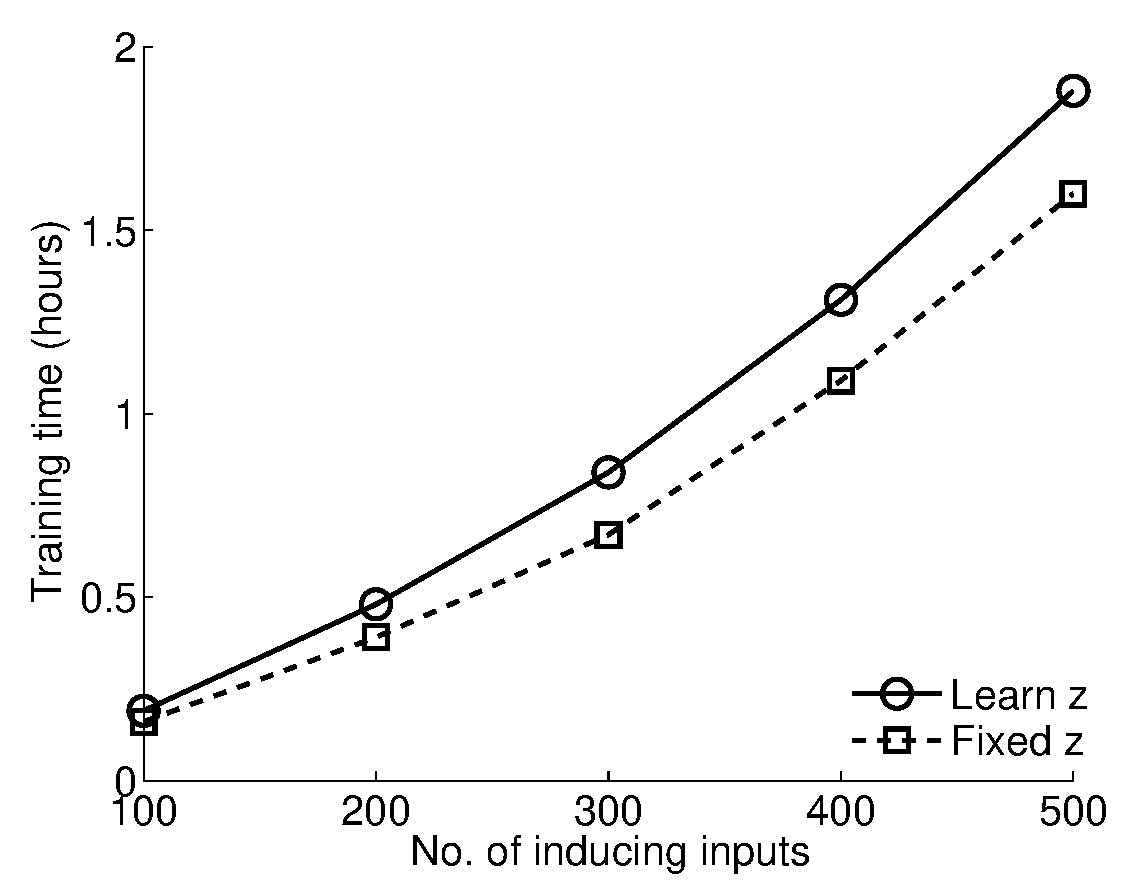
\includegraphics[scale=0.4]{figures/sarcosTime.eps}
\caption{The cost of optimizing versus fixing the inducing inputs.}
\label{fig:time}
\end{figure}
